% \chapter{System Overview and Data Pipeline}
% \label{chap:pipeline}

% This chapter describes the end-to-end pipeline that turns raw Indian
% court-judgment text into a labelled, leakage-audited, heterogeneous
% knowledge graph ready for Graph Neural Network (GNN) training. The
% pipeline was designed around three practical constraints: (i) the corpus
% is large and noisy, so every stage is a batch process with explicit
% caching and auditing; (ii) many of the signals a predictor would want
% (decisions, dispositions, operative paragraphs) are precisely the signals
% a legally honest experiment must remove, so leakage prevention has to be
% baked in rather than bolted on; and (iii) the downstream target is a
% graph, so text extraction and entity resolution have to produce outputs
% that can be reified as typed nodes and edges without lossy renormalisation
% later on.

% \section{System Architecture Overview}

% The system is organised as a six-stage pipeline. Each stage is an
% independently re-runnable batch process; intermediate artefacts are
% cached on disk so that an expensive step (OpenNyAI NER on tens of
% thousands of judgments, or bge-m3 embedding on millions of text spans)
% never has to be repeated when a later stage changes.

% \begin{figure}[H]
%   \centering
%   \begin{tikzpicture}[
%       node distance=0.45cm and 0.7cm,
%       every node/.style={font=\small},
%       stage/.style={rectangle, rounded corners, draw=black!70, thick,
%         fill=blue!6, minimum width=4.2cm, minimum height=0.95cm,
%         align=center, text width=4.1cm},
%       artefact/.style={rectangle, draw=black!40, dashed, fill=gray!4,
%         minimum width=4.2cm, minimum height=0.7cm, align=center,
%         text width=4.1cm, font=\footnotesize\itshape},
%       arrow/.style={-{Stealth[length=2mm]}, thick}
%     ]
%     \node[stage] (s1) {\textbf{1. Document Collection}\\raw judgment
%       \texttt{.txt} files};
%     \node[artefact, below=of s1] (a1) {per-bucket raw corpora
%       (5 legal domains)};
%     \node[stage, below=of a1] (s2) {\textbf{2. OpenNyAI NER + RR}\\
%       Legal NER, Rhetorical Roles, Summariser};
%     \node[artefact, below=of s2] (a2) {enriched JSON: annotated spans,
%       RR labels, summary};
%     \node[stage, below=of a2] (s3) {\textbf{3. Mistral Outcome
%       Labelling}\\case-level win/loss/neutral + score};
%     \node[artefact, below=of s3] (a3) {\texttt{*\_timed\_mistral}
%       case JSONs};
%     \node[stage, right=3.2cm of s1] (s4) {\textbf{4. Multi-Hearing
%       Merging}\\fold earlier hearings into the final decision};
%     \node[artefact, below=of s4] (a4) {\texttt{*\_MERGED.json} final
%       case records};
%     \node[stage, below=of a4] (s5) {\textbf{5. Leakage-Safe
%       Cleaning}\\drop decision fields, mask phrases, filter RR labels};
%     \node[artefact, below=of s5] (a5) {cleaned
%       \texttt{CleanedCase} objects};
%     \node[stage, below=of a5] (s6) {\textbf{6. Graph Construction +
%       bge-m3 Encoding}\\PyG \texttt{HeteroData} + text embeddings};
%     \node[artefact, below=of s6] (a6) {per-bucket + cross-bucket
%       graph caches};
%     \draw[arrow] (s1) -- (a1);
%     \draw[arrow] (a1) -- (s2);
%     \draw[arrow] (s2) -- (a2);
%     \draw[arrow] (a2) -- (s3);
%     \draw[arrow] (s3) -- (a3);
%     \draw[arrow] (a3.east) -- ++(0.8,0) |- (s4.west);
%     \draw[arrow] (s4) -- (a4);
%     \draw[arrow] (a4) -- (s5);
%     \draw[arrow] (s5) -- (a5);
%     \draw[arrow] (a5) -- (s6);
%     \draw[arrow] (s6) -- (a6);
%   \end{tikzpicture}
%   \caption{The six-stage data pipeline. Solid boxes are processing
%   stages; dashed boxes are cached on-disk artefacts that feed the next
%   stage.}
%   \label{fig:pipeline}
% \end{figure}

% Stages~1--3 are \emph{textual enrichment}: they turn plain text into a
% structured JSON record with entities, rhetorical-role spans, and a
% case-level outcome label. Stage~4 reconciles the fact that a single
% legal matter often produces multiple hearing documents, so that each
% final case corresponds to one legal dispute rather than one PDF. Stage~5
% is a leakage-safety gate: it explicitly removes the fields, sections,
% and phrases that would let a model trivially recover the outcome.
% Stage~6 reifies the cleaned records as a typed heterogeneous graph and
% attaches pre-computed \texttt{bge-m3} text embeddings to every text
% node. Chapter~\ref{chap:kg} details the schema produced by stage~6.

% \section{Document Collection and Legal Domains}

% \emph{(Document collection methodology -- sources, filters, deduplication
% -- to be described in a later revision.)}

% The collected corpus is organised into five \textbf{legal domain
% buckets}, chosen so that each bucket is large enough to train a
% domain-specific graph and internally coherent in terms of statutory
% framework, party structure, and typical remedies. The buckets are:

% \begin{itemize}
%   \item \textbf{Family \& Matrimonial} (\texttt{family\_matrimonial\_timed\_mistral}):
%     matrimonial disputes, maintenance, custody, and dowry-related
%     proceedings. Dominated by IPC~498A, Sections~482, 506, and the CrPC.
%   \item \textbf{Financial Fraud} (\texttt{fin\_fraud\_timed\_mistral}):
%     cheating, forgery, dishonour, and economic offences. Dominated by
%     IPC~420, 468, 471.
%   \item \textbf{Land \& Property} (\texttt{land\_property\_timed\_mistral}):
%     land acquisition, title, and property disputes. Dominated by the
%     Land Acquisition Act~1894 and the Constitution of India.
%   \item \textbf{Motor Accidents} (\texttt{motor\_accidents\_timed\_mistral}):
%     compensation claims and related appeals. Dominated by the Motor
%     Vehicles Act~1988 and Section~166.
%   \item \textbf{Sexual Offences} (\texttt{sexual\_offences\_timed\_mistral}):
%     offences against the person, including POCSO matters. Dominated by
%     the IPC, CrPC, and POCSO Act.
% \end{itemize}

% Every downstream artefact -- entity canonicalisation tables,
% rhetorical-role annotations, outcome labels, and graph caches -- is
% produced both per bucket and in a unified \emph{cross-bucket} view.
% This two-level organisation is what later makes cross-domain transfer
% and cross-bucket bridge analysis possible
% (Chapter~\ref{chap:graph_exploration}).

% \section{Named Entity Recognition and Rhetorical Role Classification}

% \subsection{The OpenNyAI Pipeline}

% Textual enrichment is performed with the OpenNyAI legal NLP stack,
% running locally on GPU. The production configuration uses:

% \begin{itemize}
%   \item \texttt{Legal NER} with
%     \texttt{ner\_model\_name="en\_legal\_ner\_trf"}, sentence-level
%     inference (\texttt{ner\_do\_sentence\_level=True}) and the built-in
%     post-processor (\texttt{ner\_do\_postprocess=True});
%   \item \texttt{Rhetorical\_Role} classification, assigning each
%     sentence a legal discourse label (\textsc{Preamble}, \textsc{Facts},
%     \textsc{Arguments}, \textsc{Ratio}, \textsc{RPC}, etc.);
%   \item \texttt{Summarizer} executed after rhetorical-role
%     classification, which produces the section-structured summary
%     (\textsc{Preamble}, \textsc{facts}, \textsc{arguments}, and a
%     decision block that is later discarded).
% \end{itemize}

% The environment is pinned (spaCy~3.2.4, pydantic~1.7.4,
% CUDA-enabled PyTorch and CuPy) and run GPU-only: silent CPU fallback is
% disabled so that a broken GPU configuration fails fast rather than
% silently degrading throughput. All model caches are redirected into
% project-local folders so that re-runs do not contaminate
% \texttt{\$HOME}. Each input judgment yields a combined JSON with NER
% annotations, rhetorical-role spans, and the summary.

% \subsection{Entity Types and Their Graph Roles}

% OpenNyAI's legal NER tags span several coarse types; the ones we reify
% as graph nodes are:

% \begin{itemize}
%   \item \textsc{Statute} and \textsc{Provision} -- statutes (e.g.\ IPC,
%     CrPC, Motor Vehicles Act) and their sections (e.g.\ Section~482).
%     Provisions are additionally linked to their parent statute via a
%     \texttt{belongs\_to\_statute} edge.
%   \item \textsc{Precedent} -- cited case references.
%   \item \textsc{Court} and \textsc{Judge} -- the court the matter is
%     heard in and the presiding bench.
%   \item \textsc{Petitioner}, \textsc{Respondent},
%     \textsc{Petitioner\_Lawyer}, \textsc{Defence\_Lawyer},
%     \textsc{Lawyer} -- typed party and counsel roles. Role assignment
%     uses the section in which the mention first appears (preamble vs.\
%     argument blocks) combined with OpenNyAI's entity labels.
%   \item \textsc{Org}, \textsc{GPE}, \textsc{Date}, \textsc{Case\_Number}
%     -- auxiliary types extracted by NER, retained in the cleaned JSON
%     but excluded from the final reasoning-focused graph
%     (Section~\ref{sec:graph_schema}).
% \end{itemize}

% Entities are canonicalised per bucket: surface forms are normalised
% (case, whitespace, punctuation), grouped, and re-projected as
% \texttt{canonical\_name}. Canonicalisation is what allows the same
% statute or court to be a \emph{single shared node} across the thousands
% of cases that mention it, which is the structural property that makes
% the graph useful for cross-case reasoning.

% \subsection{Rhetorical Role Taxonomy and Leakage-Safe Filtering}

% OpenNyAI's rhetorical-role taxonomy is the hinge on which the
% leakage-safety story turns. Of the labels produced by the RR model, two
% are inherently decisive -- \textbf{RPC} (Ratio and Precedent Cited, in
% practice the court's operative paragraph) and \textbf{RLC} (Ruling by
% Lower Court). Keeping either of them would let a classifier read the
% outcome verbatim.

% The cleaning stage therefore treats both labels as
% \texttt{FORBIDDEN\_ANNOTATION\_LABELS}: any annotation whose label set
% intersects \{\textsc{RPC}, \textsc{RLC}\} is dropped outright, along
% with any annotation whose summary section is \textsc{decision} or whose
% label string contains \texttt{"decision"}, \texttt{"disposition"},
% \texttt{"operative"}, \texttt{"order"}, or \texttt{"rpc"}. Only the
% three non-decisive summary fields -- \textsc{Preamble},
% \textsc{facts}, and \textsc{arguments} -- are retained as text sources
% for the graph's text nodes. This is the first leakage gate; a second,
% phrase-level gate is described in Section~\ref{sec:leakage_prevention}.

% \section{Outcome Labelling with Mistral}

% \subsection{Labelling Methodology}

% Case-level outcome labels are produced by prompting a Mistral LLM with
% the OpenNyAI summary and asking it to return a structured judgement:
% a label ($\text{win} = +1$, $\text{loss} = -1$, or \textsc{neutral}),
% a confidence-weighted \texttt{outcome\_score} in $[-1, +1]$, and a short
% textual explanation. Labelling is done from the \emph{summaries
% produced by OpenNyAI}, not from the raw judgment text, so that the
% label generator sees the same content the downstream model would see
% if no leakage cleaning were applied -- which then forces us to remove
% the decision-bearing portions of that summary before training. The
% resulting artefacts are the \texttt{*\_timed\_mistral} buckets used
% throughout the rest of the thesis.

% Both single-label and multi-label variants are produced
% (\texttt{add\_case\_outcome\_labels\_mistral.py} and
% \texttt{add\_multi\_label\_outcome\_from\_enriched.py}). This work uses
% the single-label variant as the prediction target; the multi-label
% variant is kept as a diagnostic artefact.

% \subsection{Coverage and Label Distribution}

% Labelling coverage and the resulting win/loss/neutral distribution are
% summarised in Figures~\ref{fig:labelling_coverage}
% and~\ref{fig:outcome_distribution}. Coverage is near-complete across
% all five buckets; the class distribution is moderately imbalanced
% (roughly $60\%$ \textsc{win} to $40\%$ \textsc{loss} on the pooled
% cross-bucket dataset), which motivates the use of macro-F1 alongside
% accuracy as a primary metric in Chapter~\ref{chap:results}.

% \begin{figure}[H]
%   \centering
%   
\includegraphics[width=0.92\textwidth]{figures/labelling_coverage_full.png}
%   \caption{Mistral labelling coverage per bucket.}
%   \label{fig:labelling_coverage}
% \end{figure}

% \begin{figure}[H]
%   \centering
%   
\includegraphics[width=0.92\textwidth]{figures/outcome_distribution_full.png}
%   \caption{Outcome label distribution per bucket.}
%   \label{fig:outcome_distribution}
% \end{figure}

% \section{Multi-Hearing Merging}
% \label{sec:multi_hearing_merging}

% \subsection{The Problem}

% A single legal matter frequently produces more than one judgment
% document: interim orders, remands, partial disposals, and the final
% decision may all be published as separate PDFs with distinct
% Indian-Kanoon-style filenames that nonetheless refer to the same case.
% If these hearing files are fed into the graph independently, three
% things go wrong:

% \begin{enumerate}
%   \item duplicate \textsc{Case} nodes for what is actually one dispute
%     inflate the node count and double-count outcomes;
%   \item the outcome label of the final hearing is not propagated to the
%     earlier hearings, so the training signal is noisy; and
%   \item cross-case structural signals (shared parties, statutes, and
%     counsel across hearings) are double-counted as if they were
%     independent observations.
% \end{enumerate}

% \subsection{Merge Strategy}

% The merging pipeline lives under
% \texttt{Thesis\_FINAL\_DATA/TIMELINE} and
% \texttt{DATA\_SET\_BUILDER\_AND\_EXPLORER/Timeline\_Maker}. Per bucket,
% filenames are parsed into a \texttt{(title,\ hearing\_date)} tuple; the
% latest hearing becomes the \emph{final} case, and every older hearing
% with the same title is \emph{folded} into that final case's JSON. The
% fold step either appends the older document's text under a
% \texttt{prior\_hearings} block (when the final document does not
% already contain that text) or is skipped when the final document
% already subsumes it. Every merge is logged in a per-bucket
% \texttt{report.json} so the operation is auditable and reversible.

% The scale of the fold is non-trivial but concentrated:

% \begin{table}[H]
%   \centering
%   \small
%   \begin{tabular}{lrrrrr}
%     \toprule
%     Bucket & Inputs & Final cases & Folded in & Appended & Already contained \\
%     \midrule
%     Family \& Matrimonial & 15{,}800 & 15{,}306 & 493 & 490 & 3 \\
%     Financial Fraud & 15{,}014 & 14{,}615 & 399 & 396 & 3 \\
%     Land \& Property & 14{,}324 & 14{,}051 & 251 & 242 & 9 \\
%     Motor Accidents & 15{,}271 & 15{,}236 & 32 & 30 & 2 \\
%     Sexual Offences & 15{,}532 & 14{,}596 & 936 & 932 & 4 \\
%     \midrule
%     \textbf{Total} & \textbf{75{,}941} & \textbf{73{,}804} & \textbf{2{,}111}
%       & \textbf{2{,}090} & \textbf{21} \\
%     \bottomrule
%   \end{tabular}
%   \caption{Multi-hearing merge statistics. 2{,}111 older hearing
%   documents across the five buckets were folded into 2{,}090 merged
%   final-case JSONs; the remaining 21 were already fully contained in
%   the final hearing.}
%   \label{tab:merge_stats}
% \end{table}

% Sexual-offences matters fold most aggressively, which is consistent with
% their tendency to generate multiple remand and bail-stage orders before
% a final judgment; motor-accidents matters fold least, because the
% compensation process terminates in one tribunal order more often than
% it does in the other buckets.

% \section{Technology Stack}

% The pipeline is entirely Python-based. NER, RR, and summarisation run
% on top of \texttt{opennyai} with spaCy~3.2.4 and CUDA-enabled PyTorch
% and CuPy, provisioned via the pinned micromamba environment
% \texttt{fixed\_gpu\_opennyai\_final}. Outcome labelling uses a Mistral
% model invoked through a batched client script. Multi-hearing merging is
% implemented with \texttt{merge\_cases.py} and \texttt{merge\_cases\_v2.py}
% under the \texttt{Timeline\_Maker} module. Graph construction is built
% on \texttt{torch\_geometric}'s \texttt{HeteroData}, with text
% embeddings produced by the \texttt{BAAI/bge-m3} sentence-transformer
% model running multi-process on GPU and cached per bucket. Training,
% ablation, and analysis scripts live under the \texttt{section\_GNN}
% module.

\chapter{System Overview and Data Pipeline}
\label{chap:pipeline}

This chapter describes the end-to-end pipeline that turns raw Indian
court-judgment text into a labelled, leakage-audited, heterogeneous
knowledge graph ready for Graph Neural Network (GNN) training. The
pipeline was designed around three practical constraints: (i) the corpus
is large and noisy, so every stage is a batch process with explicit
caching and auditing; (ii) many of the signals a predictor would want
(decisions, dispositions, operative paragraphs) are precisely the signals
a legally honest experiment must remove, so leakage prevention has to be
baked in rather than bolted on; and (iii) the downstream target is a
graph, so text extraction and entity resolution have to produce outputs
that can be reified as typed nodes and edges without lossy renormalisation
later on.

\section{System Architecture Overview}

The system is organised as a six-stage pipeline. Each stage is an
independently re-runnable batch process; intermediate artefacts are
cached on disk so that an expensive step (OpenNyAI NER on tens of
thousands of judgments, or bge-m3 embedding on millions of text spans)
never has to be repeated when a later stage changes.

\begin{figure}[H]
  \centering
  \begin{tikzpicture}[
      node distance=0.45cm and 0.7cm,
      every node/.style={font=\small},
      stage/.style={rectangle, rounded corners, draw=black!70, thick,
        fill=blue!6, minimum width=4.2cm, minimum height=0.95cm,
        align=center, text width=4.1cm},
      artefact/.style={rectangle, draw=black!40, dashed, fill=gray!4,
        minimum width=4.2cm, minimum height=0.7cm, align=center,
        text width=4.1cm, font=\footnotesize\itshape},
      arrow/.style={-{Stealth[length=2mm]}, thick}
    ]
    \node[stage] (s1) {\textbf{1. Document Collection}\\raw judgment
      \texttt{.txt} files};
    \node[artefact, below=of s1] (a1) {per-bucket raw corpora
      (5 legal domains)};
    \node[stage, below=of a1] (s2) {\textbf{2. OpenNyAI NER + RR}\\
      Legal NER, Rhetorical Roles, Summariser};
    \node[artefact, below=of s2] (a2) {enriched JSON: annotated spans,
      RR labels, summary};
    \node[stage, below=of a2] (s3) {\textbf{3. Mistral Outcome
      Labelling}\\case-level win/loss/neutral + score};
    \node[artefact, below=of s3] (a3) {\texttt{*\_timed\_mistral}
      case JSONs};
    \node[stage, right=3.2cm of s1] (s4) {\textbf{4. Multi-Hearing
      Merging}\\fold earlier hearings into the final decision};
    \node[artefact, below=of s4] (a4) {\texttt{*\_MERGED.json} final
      case records};
    \node[stage, below=of a4] (s5) {\textbf{5. Leakage-Safe
      Cleaning}\\drop decision fields, mask phrases, filter RR labels};
    \node[artefact, below=of s5] (a5) {cleaned
      \texttt{CleanedCase} objects};
    \node[stage, below=of a5] (s6) {\textbf{6. Graph Construction +
      bge-m3 Encoding}\\PyG \texttt{HeteroData} + text embeddings};
    \node[artefact, below=of s6] (a6) {per-bucket + cross-bucket
      graph caches};
    \draw[arrow] (s1) -- (a1);
    \draw[arrow] (a1) -- (s2);
    \draw[arrow] (s2) -- (a2);
    \draw[arrow] (a2) -- (s3);
    \draw[arrow] (s3) -- (a3);
    \draw[arrow] (a3.east) -- ++(0.8,0) |- (s4.west);
    \draw[arrow] (s4) -- (a4);
    \draw[arrow] (a4) -- (s5);
    \draw[arrow] (s5) -- (a5);
    \draw[arrow] (a5) -- (s6);
    \draw[arrow] (s6) -- (a6);
  \end{tikzpicture}
  \caption{The six-stage data pipeline. Solid boxes are processing
  stages; dashed boxes are cached on-disk artefacts that feed the next
  stage.}
  \label{fig:pipeline}
\end{figure}

Stages~1--3 are \emph{textual enrichment}: they turn plain text into a
structured JSON record with entities, rhetorical-role spans, and a
case-level outcome label. Stage~4 reconciles the fact that a single
legal matter often produces multiple hearing documents, so that each
final case corresponds to one legal dispute rather than one PDF. Stage~5
is a leakage-safety gate: it explicitly removes the fields, sections,
and phrases that would let a model trivially recover the outcome.
Stage~6 reifies the cleaned records as a typed heterogeneous graph and
attaches pre-computed \texttt{bge-m3} text embeddings to every text
node. Chapter~\ref{chap:kg} details the schema produced by stage~6.

\section{Document Collection and Legal Domains}

{
\subsection{Source Selection and Crawling Strategy}

\begin{sloppypar}
The data source for the underlying judgments is Indian Kanoon (\texttt{indiankanoon.org}). It was selected for its comprehensive, publicly accessible archive of Indian High Court judgments and its semi-structured search interface, which is uniquely suited for programmatic access compared to proprietary databases. However, accessing a deep, historical sample from the platform involves structural challenges. Indian Kanoon's search results for any single query are practically truncated at a cap of 40 pages (approximately 400 accessible documents) per search window. 
\end{sloppypar}

\begin{sloppypar}
To overcome this truncation, data collection was structured around discrete \emph{court-month windows}. For each target High Court and for each calendar month across the target years, the scraper executed an explicitly bounded query (e.g., \path{doctypes:<court> fromdate:1-<month>-<year> todate:<last_day>-<month>-<year>}). By narrowing the temporal bounds to a single month per jurisdiction, the total number of judgments returned per window consistently stayed within the access limits, allowing for an exhaustive download of the raw corpus without relying on single broad keyword queries. The judgments were initially collected and stored directly in their raw PDF format. Furthermore, no deduplication methodologies were employed on the text or case level beyond a basic check to prevent re-downloading the same numeric Indian Kanoon document ID.
\end{sloppypar}

\subsection{Local Bucketing and Legal Domains}

Rather than trusting black-box search engines to selectively define the corpus---which could bias the dataset towards heavily-cited ``landmark'' cases while omitting routine baseline cases---the classification of documents into specific legal domains was implemented locally as a deterministic post-processing step.

After downloading the entire accessible window, each raw PDF underwent text extraction (via PyMuPDF) and was passed through a local filtering script. This script evaluated the text against a rigid set of regular expressions corresponding to required statutory provisions (e.g., ``Section 498A IPC'', ``Motor Vehicles Act'', ``POCSO'') and contextual keyword constraints. Scraped texts that successfully matched a domain's predefined rules were partitioned into the respective local directory buckets.

The collected corpus resulting from this process is organised into five \textbf{legal domain buckets}, chosen so that each bucket is large enough to train a domain-specific graph and internally coherent in terms of statutory framework, party structure, and typical remedies. The buckets are:
}

\begin{itemize}
  \item \textbf{Family \& Matrimonial} (\path{family_matrimonial_timed_mistral}):
    matrimonial disputes, maintenance, custody, and dowry-related
    proceedings. Dominated by IPC~498A, Sections~482, 506, and the CrPC.
  \item \textbf{Financial Fraud} (\path{fin_fraud_timed_mistral}):
    cheating, forgery, dishonour, and economic offences. Dominated by
    IPC~420, 468, 471.
  \item \textbf{Land \& Property} (\path{land_property_timed_mistral}):
    land acquisition, title, and property disputes. Dominated by the
    Land Acquisition Act~1894 and the Constitution of India.
  \item \textbf{Motor Accidents} (\path{motor_accidents_timed_mistral}):
    compensation claims and related appeals. Dominated by the Motor
    Vehicles Act~1988 and Section~166.
  \item \textbf{Sexual Offences} (\path{sexual_offences_timed_mistral}):
    offences against the person, including POCSO matters. Dominated by
    the IPC, CrPC, and POCSO Act.
\end{itemize}

A key design requirement for domain-bucketed training is that no single
domain dominates the corpus: a strongly size-imbalanced corpus would
confound cross-domain accuracy comparisons, attributing performance
differences to sample-size effects rather than to genuine legal-domain
structure. Figure~\ref{fig:case_counts} verifies that the five buckets
are broadly comparable after multi-hearing merging, with all domains
falling between approximately 14{,}000 and 15{,}000 final cases. The
near-equal scale means that cross-bucket aggregation is a fair average
rather than an average skewed by one large domain.

\begin{figure}[H]
  \centering
  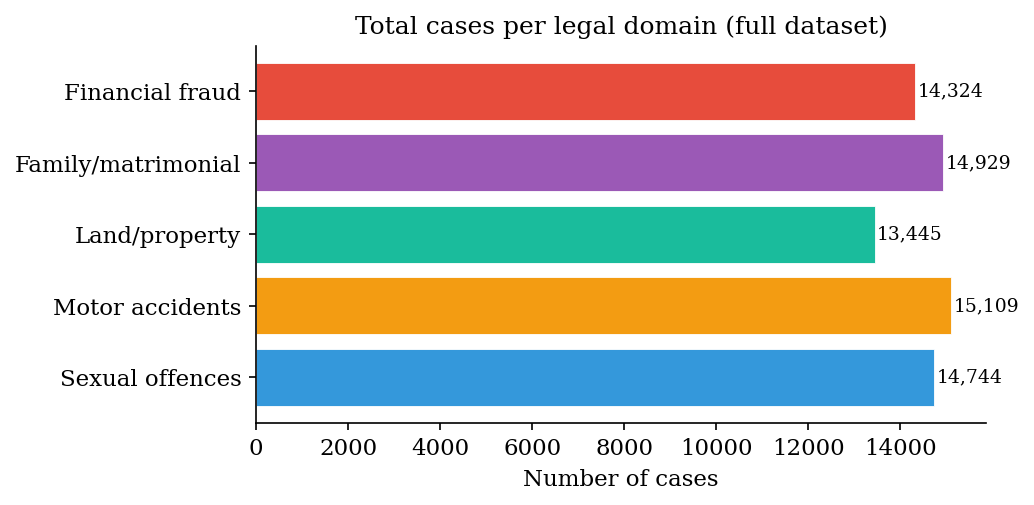
\includegraphics[width=0.92\textwidth]{figures/01_case_counts_full.png}
  \caption{Final case counts per legal domain bucket after multi-hearing
  merging. All five buckets are within a 10\% range of each other,
  confirming that the corpus is balanced at the domain level and that
  cross-bucket performance comparisons are not confounded by sample-size
  differences.}
  \label{fig:case_counts}
\end{figure}

Every downstream artefact -- entity canonicalisation tables,
rhetorical-role annotations, outcome labels, and graph caches -- is
produced both per bucket and in a unified \emph{cross-bucket} view.
This two-level organisation is what later makes cross-domain transfer
and cross-bucket bridge analysis possible
(Chapter~\ref{chap:graph_exploration}).

\section{Named Entity Recognition and Rhetorical Role Classification}
\label{sec:ner_rr}

Before a judgment can enter the knowledge graph, its raw text must be decomposed
into typed, structured units: named legal entities tied to precise character
positions, a discourse-level rhetorical role assigned to each sentence, and a
section-structured summary that separates the preamble, factual background, party
arguments, and operative ruling. For this enrichment step we use the OpenNyAI
legal NLP stack. The rationale is threefold. First, OpenNyAI's NER model was
trained specifically on Indian court judgments and recognises entity types that
a general-purpose tagger misses entirely: statutory provisions cited in the Indian
Parliament style, case precedents in the AIR/SCC citation format, and distinct
party roles such as \textsc{Petitioner}, \textsc{Respondent}, and
\textsc{Defence Lawyer}. Second, its rhetorical-role classifier is trained on the
discourse conventions of Indian High Court judgments, which differ substantially
from the conventions of news or scientific text. Third, running the stack locally
on GPU gives full control over caching and reproducibility, which is essential
when the pipeline may need to be rerun as the graph schema or leakage-cleaning
rules evolve. The following subsections describe the implementation, the output
fields produced at each stage, and how those fields feed into graph construction
and leakage removal.

\subsection{The OpenNyAI Pipeline}

Three OpenNyAI components are run in sequence for every judgment document.

\begin{itemize}
  \item \textbf{Legal NER} (\path{en_legal_ner_trf}), configured with
    sentence-level inference (\path{ner_do_sentence_level=True}) and built-in
    post-processing (\path{ner_do_postprocess=True}), tags named entities by
    type and normalises them to canonical surface forms.
  \item \textbf{Rhetorical Role Classifier} assigns each sentence one of seven
    discourse labels reflecting its function within the judgment
    (\textsc{Preamble}, \textsc{Facts}, \textsc{Arguments}, \textsc{Ratio},
    \textsc{RPC}, \textsc{RLC}, and \textsc{None}).
  \item \textbf{Summarizer}, conditioned on the predicted rhetorical roles,
    produces a section-structured extractive summary with four named blocks:
    \textsc{Preamble}, \textsc{facts}, \textsc{arguments}, and
    \textsc{decision}.
\end{itemize}

The environment is pinned (spaCy~3.2.4, pydantic~1.7.4, CUDA-enabled PyTorch
and CuPy) and run GPU-only: silent CPU fallback is disabled so that a broken GPU
configuration fails fast rather than silently degrading throughput. All model
caches are redirected into project-local folders. Each input judgment produces a
single combined JSON record that is extended by every subsequent pipeline stage.

Table~\ref{tab:pipeline_fields} lists every field written by the three OpenNyAI
components, together with the fields added by the Mistral outcome labeller
described in Section~\ref{sec:mistral_labelling}. Subsequent subsections explain
the semantic role of each field.

{\small
\setlength{\tabcolsep}{4pt}
\begin{longtable}{@{}L{2.0cm}L{3.8cm}L{6.9cm}@{}}
  \caption{Fields produced at each stage of the enrichment pipeline. All fields
  are stored in a single per-judgment JSON record, extended at each successive
  stage. The \textsc{decision} summary field is the only field not propagated to
  the final graph: it is consumed by the Mistral labeller and then removed.}
  \label{tab:pipeline_fields} \\
  \toprule
  Stage & Field & Description \\
  \midrule
  \endfirsthead
  \caption[]{Fields produced at each stage of the enrichment pipeline (continued).} \\
  \toprule
  Stage & Field & Description \\
  \midrule
  \endhead
  \bottomrule
  \endfoot
  \bottomrule
  \endlastfoot
  \multicolumn{3}{@{}l}{\textit{Legal NER}} \\[2pt]
   & \path{entity.text}
     & Surface form of the named entity as it appears in the source text. \\
   & \path{entity.label}
     & Entity type: \textsc{Statute}, \textsc{Provision}, \textsc{Precedent},
       \textsc{Court}, \textsc{Judge}, \textsc{Petitioner},
       \textsc{Respondent}, \textsc{Lawyer}, \textsc{Org}, \textsc{GPE},
       \textsc{Date}, or \textsc{Case\_Number}. \\
   & \path{entity.normalized_name}
     & Canonical form after post-processing: case-folded,
       whitespace-collapsed, and deduplicated within the document. \\
   & \path{entity.start/end}
     & Character offsets into the judgment text, used to anchor entities to
       sentences and produce aligned graph edges. \\
   & \path{unique_statutes}
     & Document-level deduplicated list of all statute canonical names. \\
   & \path{unique_provisions}
     & Document-level deduplicated list of all provision canonical names. \\
   & \path{unique_precedents}
     & Document-level deduplicated list of all cited precedent names. \\[4pt]
  \multicolumn{3}{@{}l}{\textit{Rhetorical Role Classifier}} \\[2pt]
   & \path{sentence.rhetorical_role}
     & Per-sentence discourse label: \textsc{Preamble}, \textsc{Facts},
       \textsc{Arguments}, \textsc{Ratio}, \textsc{RPC} (ratio and precedent
       cited), \textsc{RLC} (ruling by lower court), or \textsc{None}. \\
   & \path{role_counts}
     & Document-level frequency of each rhetorical role, used for corpus
       analysis and leakage auditing. \\[4pt]
  \multicolumn{3}{@{}l}{\textit{Summarizer}} \\[2pt]
   & \path{opennyai_summary.PREAMBLE}
     & Extractive summary of the preamble block: court name, bench
       composition, case registration number, and party names. \\
   & \path{opennyai_summary.facts}
     & Extractive summary of the factual background sentences. \\
   & \path{opennyai_summary.arguments}
     & Extractive summary of arguments advanced by both parties. \\
   & \path{opennyai_summary.decision}
     & Extractive summary of the operative ruling. Read by the Mistral
       labeller and then discarded before graph construction to prevent
       outcome leakage. \\[4pt]
  \multicolumn{3}{@{}l}{\textit{Mistral Outcome Labeller}} \\[2pt]
   & \path{case_outcome_label}
     & Categorical outcome from the appellant's perspective:
       \path{appellant_won}, \path{appellant_lost}, or
       \path{postponed_or_procedural}. \\
   & \path{case_outcome_score}
     & Numeric encoding of the label: $+1$ (won), $-1$ (lost), $0$
       (procedural). \\
   & \path{llm_case_outcome.confidence}
     & Model-reported classification confidence: \path{high},
       \path{medium}, or \path{low}. \\
   & \path{llm_case_outcome.short_explanation}
     & One or two sentence rationale produced alongside the label,
       retained for manual auditing. \\
\end{longtable}
}

\subsection{Entity Types and Their Graph Roles}

OpenNyAI's legal NER recognises twelve entity types; the subset reified as graph
nodes in the downstream knowledge graph is:

\begin{sloppypar}
\begin{itemize}
  \item \textsc{Statute} and \textsc{Provision}: statutes (e.g.\ the IPC,
    the CrPC, the Motor Vehicles Act) and their sections (e.g.\ Section~482).
    Provisions are additionally linked to their parent statute via a
    \texttt{belongs\_to\_statute} edge.
  \item \textsc{Precedent}: cited case references.
  \item \textsc{Court} and \textsc{Judge}: the court the matter is heard in
    and the presiding bench.
  \item \textsc{Petitioner}, \textsc{Respondent},
    \textsc{Petitioner\_Lawyer}, \textsc{Defence\_Lawyer}, \textsc{Lawyer}:
    typed party and counsel roles. Role assignment uses the section in which
    the mention first appears (preamble versus argument blocks) combined with
    OpenNyAI's entity labels.
  \item \textsc{Org}, \textsc{GPE}, \textsc{Date}, \textsc{Case\_Number}:
    auxiliary types extracted by NER, retained in the cleaned JSON but excluded
    from the final reasoning-focused graph (Section~\ref{sec:graph_schema}).
\end{itemize}
\end{sloppypar}

Entities are canonicalised per bucket: surface forms are normalised (case,
whitespace, punctuation), grouped, and re-projected as \texttt{canonical\_name}.
Canonicalisation allows the same statute or court to appear as a \emph{single
shared node} across the thousands of cases that mention it, which is the
structural property that makes the graph useful for cross-case reasoning.

To verify that the extraction stage is producing entity distributions consistent
with the legal character of each domain, Figure~\ref{fig:entity_type_totals}
summarises the total entity mention counts by type across the full corpus. The
figure shows that precedents dominate in absolute volume, confirming that citation
is the primary relational artefact in Indian court judgments. Party nodes
(\textsc{Petitioner} and \textsc{Respondent}) are large and roughly equal in
volume across the corpus as a whole, reflecting the adversarial structure of
litigation. Statutes and provisions, by contrast, have comparatively lower raw
mention counts but are the node types that carry the most cross-case structural
weight: each canonicalised mention is a potential shared edge linking the current
case to every other case that cites the same authority. This asymmetry between
volume and structural importance is what motivates treating statutes, provisions,
and precedents as the shared layer of the graph while keeping party nodes local
to each case.

\begin{figure}[H]
  \centering
  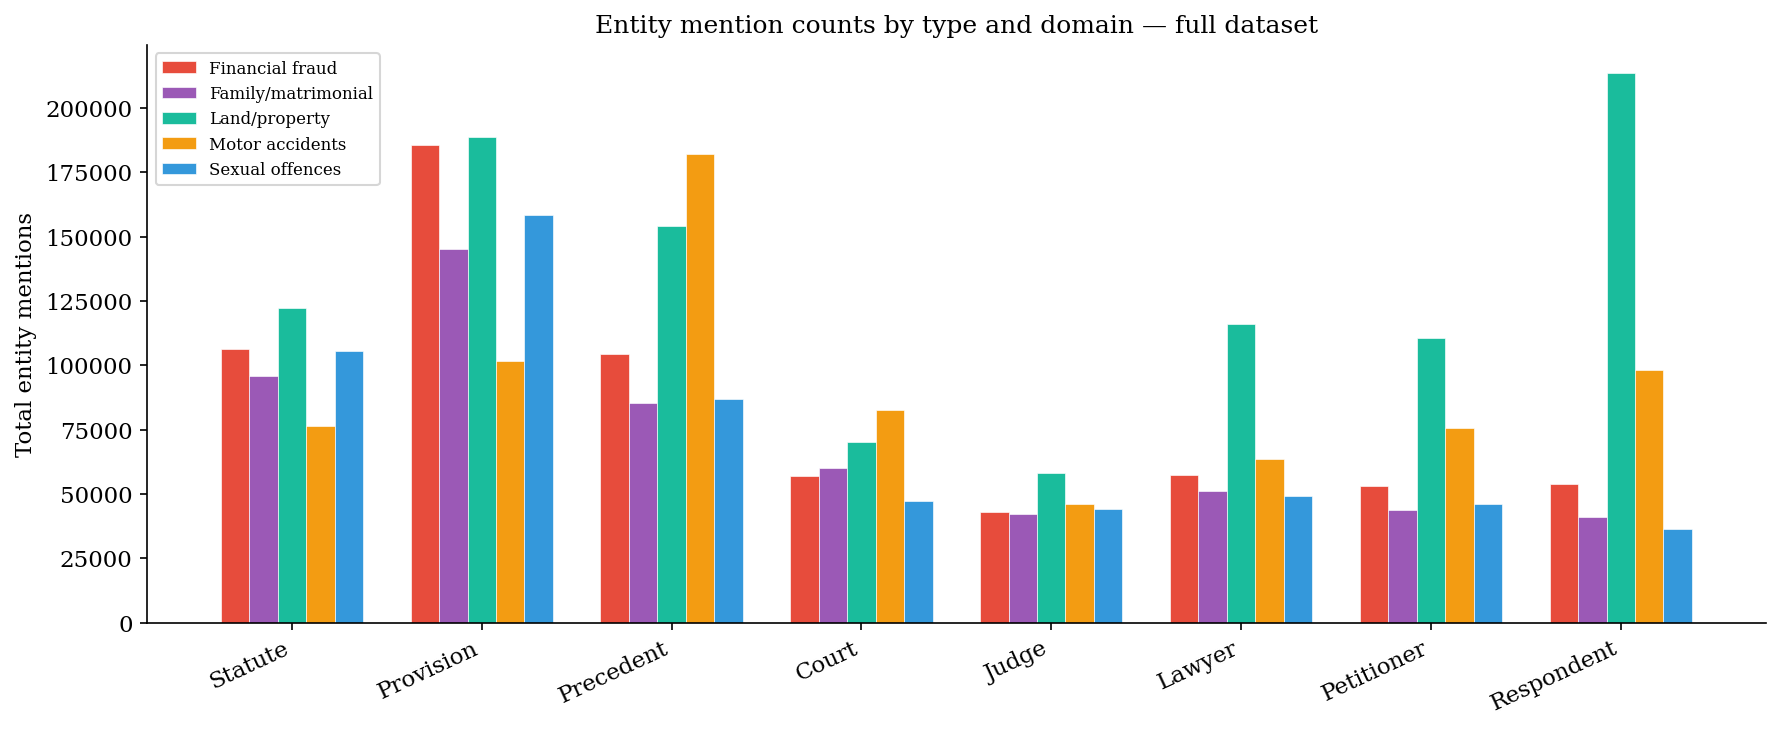
\includegraphics[width=0.92\textwidth]{figures/04_entity_type_totals_full.png}
  \caption{Total entity mention counts by type across the full corpus after
  NER and canonicalisation. Precedent mentions dominate in volume; statutes
  and provisions are smaller in count but form the shared-node layer that
  carries structural weight across cases.}
  \label{fig:entity_type_totals}
\end{figure}

\subsection{Rhetorical Role Taxonomy and Leakage-Safe Filtering}

OpenNyAI's rhetorical-role taxonomy is the hinge on which the leakage-safety
story turns. Of the seven labels produced by the classifier, two are inherently
decisive: \textbf{RPC} (Ratio and Precedent Cited, in practice the court's
operative paragraph) and \textbf{RLC} (Ruling by Lower Court). Keeping either
of them in the training data would let a classifier read the outcome directly
from the text.

The cleaning stage therefore treats both labels as forbidden annotation labels:
any annotation whose label set intersects \{\textsc{RPC}, \textsc{RLC}\} is
dropped outright, along with any annotation whose summary section is
\textsc{decision} or whose label string contains \texttt{"decision"},
\texttt{"disposition"}, \texttt{"operative"}, \texttt{"order"}, or
\texttt{"rpc"}. Only the three non-decisive summary fields (\textsc{Preamble},
\textsc{facts}, and \textsc{arguments}) are retained as text sources for the
graph's text nodes. This is the first leakage gate; a second, phrase-level gate
is described in Section~\ref{sec:leakage_prevention}.

\section{Outcome Labelling with Mistral}
\label{sec:mistral_labelling}

With judgments enriched by NER and rhetorical-role annotations, the next
requirement is a case-level outcome label: did the appellant win, lose, or
receive only a procedural disposition? We produce these labels automatically by
prompting a Mistral large language model with the section-structured summaries
that OpenNyAI already generates. This approach has two important properties.
First, the model is shown only the \textsc{decision} summary block and the
\textsc{RPC} sentences, which are precisely the portions that the
leakage-cleaning stage will subsequently remove. The labeller therefore never
sees the non-decisive preamble, facts, or arguments text that the GNN will train
on, eliminating any circularity between what gets labelled and what gets learned.
Second, the section-structured input provides a compact, well-delimited context
that substantially reduces the chance that the model grounds its judgement on
spurious signals from the surrounding narrative.

\subsection{Labelling Methodology}
\label{sec:labelling_methodology}

\paragraph{Labels.}
Three outcome categories are defined from the perspective of the party seeking
relief (the appellant, petitioner, or applicant):

\begin{itemize}
  \item \textbf{\texttt{appellant\_won}} ($\texttt{score} = +1$): relief was
    granted, the petition or appeal was allowed, bail was granted, a conviction
    was quashed, or an order was set aside.
  \item \textbf{\texttt{appellant\_lost}} ($\texttt{score} = -1$): the petition,
    appeal, or application was dismissed, rejected, or denied; bail was refused;
    or relief was withheld.
  \item \textbf{\texttt{postponed\_or\_procedural}} ($\texttt{score} = 0$): the
    matter was adjourned, notice was issued, a liberty was granted to pursue
    another remedy, the case was remanded, or the outcome cannot reasonably be
    treated as a final win or loss.
\end{itemize}

For each judgment the model also returns a \texttt{confidence} rating
(\texttt{high}, \texttt{medium}, or \texttt{low}) and a short textual
explanation, both stored alongside the label for auditing purposes.

\paragraph{Label model hallucination and the motivation for cross-validation.}
A known limitation of LLM-based labelling is run-to-run inconsistency. Because
language models operate with temperature sampling, the same input can yield
different labels on different inference runs. In a labelling pipeline this is a
form of hallucination with direct downstream consequences: if a substantial
fraction of the training signal is run-dependent noise rather than a reflection
of legal content, any structure a GNN learns may be an artefact of labelling
variance rather than genuine legal reasoning. The risk is sharpest for procedural
dispositions, which a model may classify as either
\texttt{postponed\_or\_procedural} or \texttt{appellant\_lost} depending on minor
wording differences between runs.

\paragraph{Cross-validation design.}
To measure this risk we ran a second independent labelling pass over the same
corpus. Crucially, the cross-validation pass uses a fundamentally different prompt
design to the original pass, removing a further source of variance: rather than
asking the model to return a single free-form label, the cross-validation prompt
decomposes the classification into six binary yes/no questions organised into two
directional signal groups, plus a two-question neutrality clause that takes
priority over all directional evidence. Table~\ref{tab:crossval_questions}
lists all eight questions.

\begin{table}[H]
  \centering
  \small
  \setlength{\tabcolsep}{4pt}
  \begin{tabular}{@{}L{3.0cm}>{\centering\arraybackslash}p{0.8cm}L{7.2cm}@{}}
    \toprule
    Group & ID & Question \\
    \midrule
    \textbf{A: Win signals}
      & Q1 & Did the appellant win the case? \\
      & Q2 & Was the petition, appeal, or application allowed? \\
      & Q3 & Did the court rule in favour of the petitioner or appellant? \\[4pt]
    \textbf{B: Loss signals}
      & Q4 & Did the respondent win the case? \\
      & Q5 & Was the petition, appeal, or application dismissed? \\
      & Q6 & Did the court rule against the appellant? \\[4pt]
    \shortstack[l]{\textbf{C: Neutrality}\\\textbf{clause}}
      & Q7 & Was the case adjourned, remanded, or deferred without a final decision? \\
      & Q8 & Is there no clear final judgment in this case? \\
    \bottomrule
  \end{tabular}
  \caption{The eight binary yes/no questions posed to the model in a single call
  during the cross-validation pass. Questions Q1--Q6 are the directional win/loss
  signals; Q7--Q8 form the neutrality clause that overrides the directional
  evidence when fired.}
  \label{tab:crossval_questions}
\end{table}

The model returns a JSON object with exactly eight integer keys (\texttt{q1}
through \texttt{q8}), each equal to 1 (yes) or 0 (no). The final label is then
determined by a fixed, deterministic aggregation rule applied to three aggregate
scores:

\[
  S_\text{win} = q_1 + q_2 + q_3, \quad
  S_\text{loss} = q_4 + q_5 + q_6, \quad
  S_\text{neutral} = q_7 + q_8.
\]

The aggregation applies the following priority ordering:

\begin{enumerate}
  \item \textbf{Neutrality clause (highest priority).} If $S_\text{neutral} > 0$
    the outcome is \texttt{postponed\_or\_procedural}, regardless of the
    directional signals. This prevents ambiguous procedural language from
    generating a spurious win or loss.
  \item \textbf{Contradiction resolution.} If both $S_\text{win} > 0$ and
    $S_\text{loss} > 0$, the majority signal wins; a tie resolves to
    \texttt{postponed\_or\_procedural} with zero confidence.
  \item \textbf{Clean classification.} If only win signals fire,
    \texttt{appellant\_won}; if only loss signals fire,
    \texttt{appellant\_lost}.
  \item \textbf{Fallback.} If all eight answers are zero, the case is marked
    \texttt{unknown} and excluded from training.
\end{enumerate}

Because the final label is computed by a deterministic function over binary
votes, the cross-validation pass eliminates the free-text generation variance
that affects the original single-label prompt. The two label sets were then
compared file-by-file using \path{compare_labels.py}, which aligns the output
directories by filename and computes per-bucket agreement rates.

\paragraph{Results.}
Across the 72{,}795 files for which both a first-pass and a cross-validation
label exist, the two independent runs agree on \textbf{84.4\%} of all cases.
The per-bucket breakdown is given in Table~\ref{tab:crossval_agreement}.

\begin{table}[H]
  \centering
  \small
  \begin{adjustbox}{max width=\textwidth}
  \begin{tabular}{lrrr}
    \toprule
    Bucket & Files compared & Matching labels & Agreement rate \\
    \midrule
    Family \& Matrimonial & 15{,}017 & 13{,}049 & 86.9\% \\
    Financial Fraud       & 14{,}342 & 12{,}015 & 83.8\% \\
    Land \& Property      & 13{,}512 &  9{,}652 & 71.4\% \\
    Motor Accidents       & 15{,}117 & 13{,}552 & 89.6\% \\
    Sexual Offences       & 14{,}807 & 13{,}143 & 88.8\% \\
    \midrule
    \textbf{Total}        & \textbf{72{,}795} & \textbf{61{,}411} & \textbf{84.4\%} \\
    \bottomrule
  \end{tabular}
  \end{adjustbox}
  \caption{Cross-run label agreement between the original Mistral pass and the
  binary-question cross-validation pass. Agreement is computed per-file over
  files present in both runs.}
  \label{tab:crossval_agreement}
\end{table}

The dominant confusion pattern is directionally consistent across buckets:
\textsc{postponed\_or\_procedural} is the primary source of disagreement,
frequently reclassified as \textsc{appellant\_lost} in the second pass. This is
most pronounced in \emph{Land \& Property}, where 2{,}927 cases originally
labelled \textsc{postponed\_or\_procedural} were relabelled
\textsc{appellant\_lost} in the cross-validation run, accounting for the bucket's
71.4\% agreement rate. The pattern is interpretable: land-property judgments
frequently conclude with procedural directions (remands, remissions to lower
courts, stay orders) that read as adverse to the appellant when examined without
full context. Notably, the neutrality clause (Q7--Q8) is designed precisely to
catch these cases; the residual disagreement reflects cases where the procedural
language is too ambiguous for even the clause to fire consistently.

The 84\% cross-run agreement establishes that label noise is real but bounded.
The ambiguous cases are disproportionately procedural dispositions rather than
clear wins or losses. For the downstream GNN, the practical consequence is that
the \textsc{postponed\_or\_procedural} class is excluded from the primary binary
prediction task (\textsc{appellant\_won} versus \textsc{appellant\_lost}). The
cross-validation agreement rate on the binary subset alone is materially higher
and sufficient to treat the first-pass labels as a reliable training signal.

\subsection{Coverage and Label Distribution}

Two questions need to be answered before trusting the label set for training.
First: did the Mistral labeller actually process every case, or are there
systematic coverage gaps? Second: is the resulting class distribution balanced
enough that a naive majority-class classifier would not trivially outperform
a learned model?

Figure~\ref{fig:labelling_coverage} addresses the first question. Coverage is
near-complete across all five buckets, with no domain showing a systematic gap.
The small number of unlabelled cases arises from Mistral returning malformed JSON
or an \texttt{unknown} fallback when the decision block is too ambiguous to
classify; these are excluded from training rather than assigned a default label.

\begin{figure}[H]
  \centering
  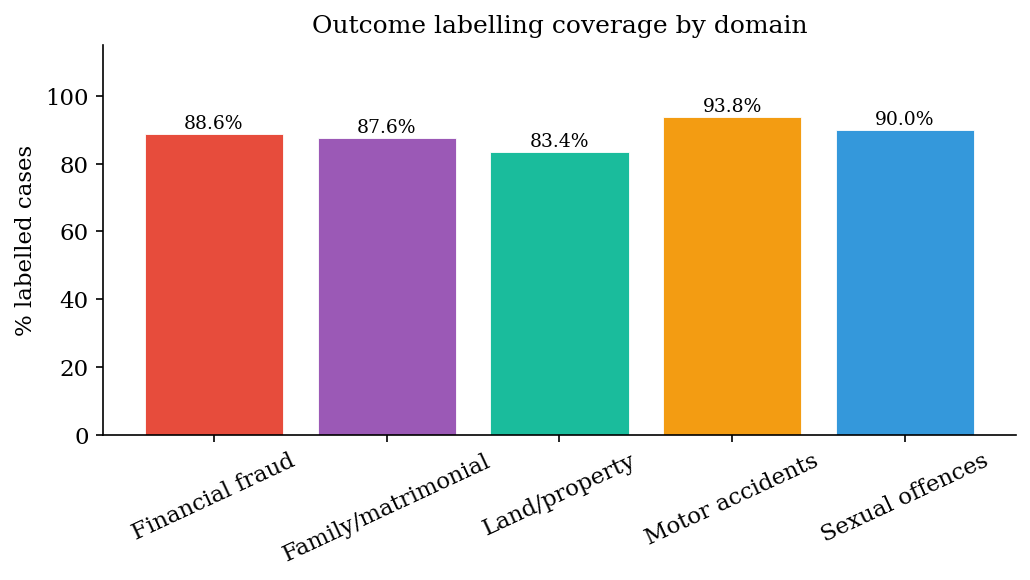
\includegraphics[width=0.92\textwidth]{figures/08_labelling_coverage_full.png}
  \caption{Mistral labelling coverage per bucket. Coverage is near-complete across
  all five domains; the small unlabelled fraction consists of cases where the
  model returned a malformed response or an explicit \texttt{unknown} verdict,
  which are excluded from training.}
  \label{fig:labelling_coverage}
\end{figure}

Figures~\ref{fig:outcome_distribution} and~\ref{fig:outcome_rate} address the
second question from complementary angles. Figure~\ref{fig:outcome_distribution}
shows raw label counts per bucket, which confirms that the procedural
(\texttt{postponed\_or\_procedural}) class is non-trivial in size but is
concentrated in certain domains. Figure~\ref{fig:outcome_rate} shows the
win/loss/neutral \emph{rates}, which makes the class-imbalance argument cleaner:
motor-accidents is the most win-skewed bucket, consistent with compensation claims
being allowed more often than denied at the appellate stage; financial-fraud sits
closest to balanced. The pooled cross-bucket win rate of roughly $60\%$
\textsc{win} to $40\%$ \textsc{loss} (on the binary subset, once procedural
cases are excluded) confirms that a constant-win classifier would achieve
misleadingly high accuracy while failing systematically on the loss class. This
is why Chapter~\ref{chap:results} reports macro-F1 alongside accuracy as a
co-primary metric.

\begin{figure}[H]
  \centering
  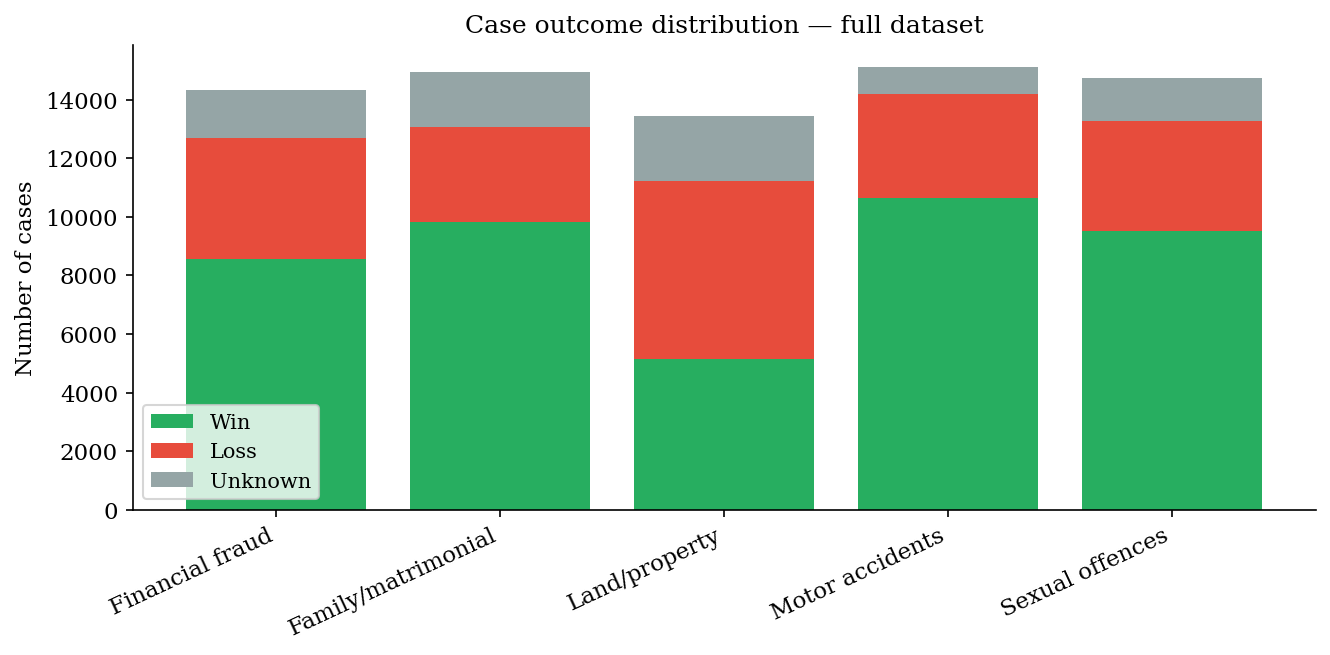
\includegraphics[width=0.92\textwidth]{figures/02_outcome_distribution_full.png}
  \caption{Absolute outcome label counts per bucket. The procedural class
  (\texttt{postponed\_or\_procedural}) is non-negligible and concentrated in
  domains where remand and interim orders are common.}
  \label{fig:outcome_distribution}
\end{figure}

\begin{figure}[H]
  \centering
  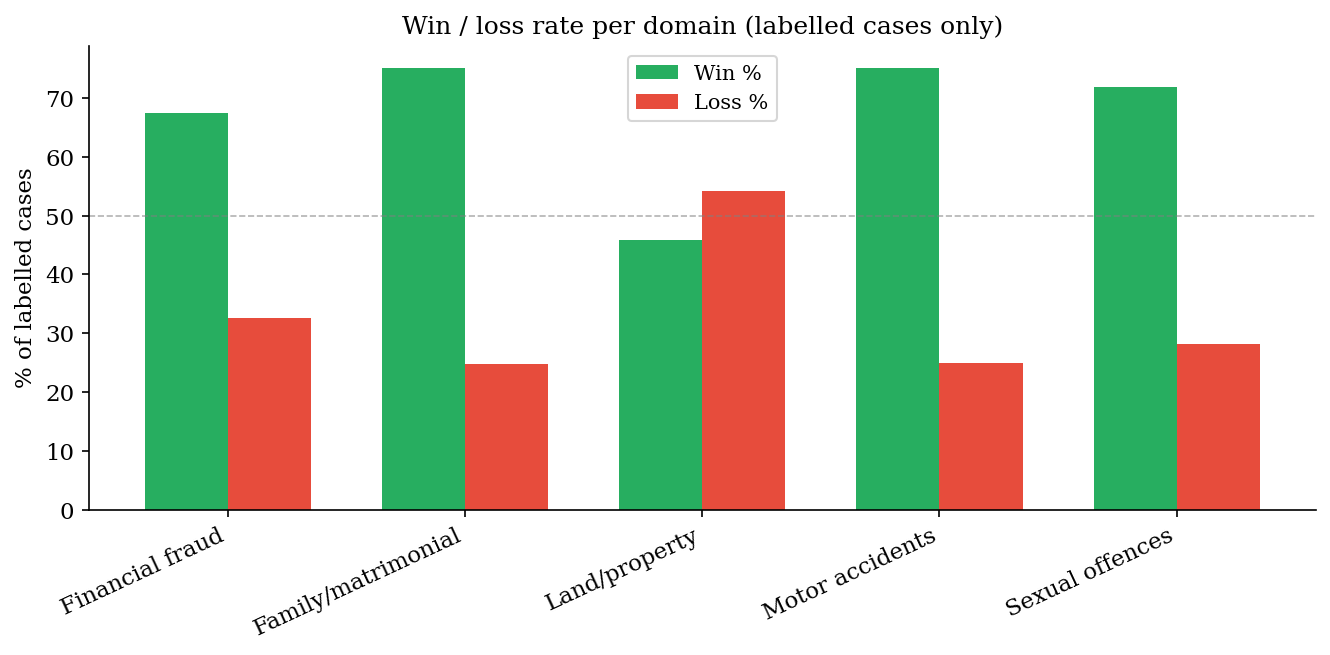
\includegraphics[width=0.92\textwidth]{figures/03_outcome_rate_full.png}
  \caption{Outcome label rates (proportions) per bucket. The rate view exposes the
  per-domain win-skew more clearly than raw counts: motor-accidents is the most
  appellant-favourable domain; financial-fraud and sexual-offences are closest to
  balanced. The cross-bucket imbalance motivates macro-F1 as the primary
  evaluation metric.}
  \label{fig:outcome_rate}
\end{figure}

\section{Multi-Hearing Merging}
\label{sec:multi_hearing_merging}

\subsection{The Problem}

A single legal matter frequently produces more than one judgment document:
interim orders, remands, partial disposals, and the final decision may all be
published as separate PDFs with distinct Indian-Kanoon-style filenames that
nonetheless refer to the same case. If these hearing files are fed into the graph
independently, three things go wrong:

\begin{enumerate}
  \item duplicate \textsc{Case} nodes for what is actually one dispute inflate
    the node count and double-count outcomes;
  \item the outcome label of the final hearing is not propagated to the earlier
    hearings, so the training signal is noisy; and
  \item cross-case structural signals (shared parties, statutes, and counsel
    across hearings) are double-counted as if they were independent observations.
\end{enumerate}

\subsection{Merge Strategy}
\label{sec:merge_strategy}

The merging pipeline is implemented in \path{merge_cases_v3.py} under
\path{DATA_SET_BUILDER_AND_EXPLORER/Timeline_Maker} and operates per bucket.
Its design reflects two iterations of lessons about what ``same case'' actually
means in a large corpus of Indian High Court judgments.

\paragraph{What the merger is and is not looking for.}
The merger is strictly interested in one type of multi-document pattern: a single
legal proceeding that was heard, adjourned, and returned to the same court on
different dates, producing a separate published judgment at each hearing stage.
The merger identifies these by the court-assigned case registration number, such
as \texttt{5941/2024} or \texttt{Crm-M-44633-2024} stamped on the preamble, and
not by any other identifier. In particular, it does \emph{not} use FIR numbers:
FIR numbers identify a police complaint rather than a court proceeding, and the
same FIR can give rise to multiple independent proceedings at different courts.
Merging on an FIR number would conflate proceedings that are legally and
factually distinct. Only documents that share both a case title (as encoded in
the Indian-Kanoon filename) \emph{and} the same court registration number are
candidates for merging.

\paragraph{The v1/v2 flaw and the v3 fix.}
Early versions of the script (\path{merge_cases.py}, \path{merge_cases_v2.py})
grouped documents by case name alone. Two litigants with the same name can appear
in genuinely unrelated proceedings spanning different courts and years, and those
proceedings can produce similarly-named judgment files. Under name-only grouping,
a pair like \emph{``Amit Kumar vs State of Bihar on 14 March, 2022''} and
\emph{``Amit Kumar vs State of Bihar on 9 November, 2024''} would be merged into
one case even if the two documents were from entirely different criminal matters.
The merged JSON would carry a single final outcome label for two unrelated cases,
directly poisoning the training signal.

The v3 script fixes this by extracting the court-assigned case registration
number from each document before grouping. Grouping is by the pair
\texttt{(case\_name,\ case\_number)}; two documents with the same name but
different registration numbers remain separate. If no registration number can be
extracted from a document, that document is kept as a standalone case and is
never merged with anything.

\paragraph{Case number extraction.}
Extraction is a three-tier search, each tier restricted to the preamble material
so that case numbers cited as precedents in the body text cannot contaminate the
identification:

\begin{enumerate}
  \item \textbf{Summary preamble.} Regex applied to the
    \texttt{PREAMBLE} entry of \path{opennyai_summary}. This is fast and covers the
    majority of documents where the summary directly contains a formatted
    registration number.
  \item \textbf{NER-sourced \textsc{Case\_Number} entities.} OpenNyAI's Legal
    NER tags \textsc{Case\_Number} spans within preamble sentences. For each
    such span the same regex normalisation is applied, with a lower minimum digit
    count, since the NER model has already confirmed the span is a case number.
  \item \textbf{Full preamble sentence text.} Regex applied to the concatenated
    text of all sentences whose rhetorical role is \textsc{Preamble}. This
    catches courts (e.g.\ Punjab~\&~Haryana) where the summary preamble is
    truncated and the registration number only appears in the sentence body.
\end{enumerate}

Seven regex patterns cover the range of registration-number formats found in the
corpus: \texttt{No./Nos.} notation (e.g.\ \texttt{No.~5941 of~2024}),
Punjab/Haryana dash-year format (e.g.\ \texttt{Crm-M-44633-2024}), CNR
alphanumeric identifiers, Delhi~HC \texttt{+}-prefixed citation lines, and a
broad three-digit-or-more slash-year fallback.

\paragraph{Merge mechanics.}
Once groups are formed, documents within each group are sorted oldest-to-latest
by hearing date. For groups with a single document, that document is written
through unchanged. For groups with the same hearing date but multiple files
(same-date duplicates), the file with the most parsed sentences is kept. For
groups with multiple distinct hearing dates, the texts are concatenated under
labelled dividers marking each earlier hearing and the final decision, and
sentence offsets are adjusted to reflect the merged linear text. The final
outcome label is always taken from the latest hearing; a containment check
suppresses duplicate text regions where the latest document already subsumes an
earlier one verbatim.

\paragraph{Scale of the operation.}
The scale of the fold is non-trivial but concentrated:

\begin{table}[H]
  \centering
  \small
  \begin{adjustbox}{max width=\textwidth}
  \begin{tabular}{lrrrrr}
    \toprule
    Bucket & Inputs & Final cases & Folded in & Appended & Already contained \\
    \midrule
    Family \& Matrimonial & 15{,}800 & 15{,}306 & 493 & 490 & 3 \\
    Financial Fraud & 15{,}014 & 14{,}615 & 399 & 396 & 3 \\
    Land \& Property & 14{,}324 & 14{,}051 & 251 & 242 & 9 \\
    Motor Accidents & 15{,}271 & 15{,}236 & 32 & 30 & 2 \\
    Sexual Offences & 15{,}532 & 14{,}596 & 936 & 932 & 4 \\
    \midrule
    \textbf{Total} & \textbf{75{,}941} & \textbf{73{,}804} & \textbf{2{,}111}
      & \textbf{2{,}090} & \textbf{21} \\
    \bottomrule
  \end{tabular}
  \end{adjustbox}
  \caption{Multi-hearing merge statistics under the case-number-aware v3
  strategy. 2{,}111 older hearing documents were folded into 2{,}090 merged
  final-case JSONs; the remaining 21 were already fully subsumed by the latest
  hearing text.}
  \label{tab:merge_stats}
\end{table}

Sexual-offences matters fold most aggressively, consistent with their tendency to
generate multiple remand and bail-stage orders before a final judgment.
Motor-accidents matters fold least, because the compensation process terminates
in a single tribunal order more often than it does in the other buckets. Every
merge is logged in a per-bucket \texttt{report.json} so the operation is
auditable and reversible.

\section{Technology Stack}

The pipeline is entirely Python-based. NER, RR, and summarisation run
on top of \texttt{opennyai} with spaCy~3.2.4 and CUDA-enabled PyTorch
and CuPy, provisioned via the pinned micromamba environment
\texttt{fixed\_gpu\_opennyai\_final}. Outcome labelling uses a Mistral
model invoked through a batched client script. Multi-hearing merging is implemented with \path{merge_cases_v3.py}
under the \path{Timeline_Maker} module. Graph construction is built
on \texttt{torch\_geometric}'s \texttt{HeteroData}, with text
embeddings produced by the \path{BAAI/bge-m3} sentence-transformer
model running multi-process on GPU and cached per bucket. Training,
ablation, and analysis scripts live under the \path{section_GNN}
module.
